\chapter{Stadiul actual în domeniu}

\section{Introducere}

\textbf{ Dezvoltarea tehnologică accelerata din ultimele decenii a afectat și domeniul educației asistate de calculator. Câteva exemple de medii accesibile publicului sunt: Second Life,  Uther Academy și iSocial (http://isocial.missouri.edu/iSocial/). Fiecare dintre aceste implementări abordeaza diferit modul livrare a materialelor educative. Deși codul sursă pentru majoritatea mediilor de învățare 3D este cod proprietar, se va încerca descrierea lor din perspectiva utilizatorului în următoarele subcapitole. Secon Life este open source și poate fi studiat. Secțiunea 3.2 se azează pe similitudini în incercarea de a determina majoritatea opțiunilor pe care un utilizator le așteapta de la mediile de învățare 3D.}


\section{Abordări similare}

\par Toate exemplele notabile prezentate ulterior fac uz de avatare pentru a induce utilizatorului sentimentul de participare activă și imersiune în lumea virtuală. Utilizatorii sunt încurajați astfel sa comunice între ei atât verbal cât și prin modificarea posturii și aparenței grafice a avatarului ce îi reprezintă în lumea virtuală.
\par Aceasta tehnică este luată în considerare în implementarea aplicației descrise în acest studiu.

\section{Second Life}
\par Percepția generală este că Second Life (SL) ar fi un joc pe Internet. Nu este însă un joc organizat, cu reguli impuse și unde să fie urmărit un anumit scop. Pe situl web oficial, Second Life este descris ca fiind „o lume virtuală imaginată și creată de rezidenții ei”; într-adevăr, SL este o lume diversificată, în care poți întâlni oameni din toate colțurile lumii reale. Este o rețea de tip social, care face parte din fenomenul din Internet numit Web 2.0.

\begin{figure}[h]
    \centering
    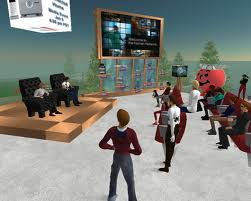
\includegraphics[]{SL}
    \caption{Eveniment în Second Life}
    \label{fig:imag3}
\end{figure}

\par Cele mai importante și interesante activități de educative sunt derulate în Second Life:
\begin{itemize}
\item Vizite asistate în muzee și teatre virtuale.
\item Cursuri în săli de clasa virtuale.
\item Jocuri de tip "orientare turistica" cu puncte intermediare și indicii cu subiect educațional.
\item Proiecte cu colaborare în echipă.
\item Cursuri online la diverse universități 
\item Panouri informative.
\item Grupuri educaționamle
\end{itemize}

\par Majoritatea facilitaților oferite de SL ar trebui să se regasească în orice platformă de e-learning cu avatare. 

\section{Uther Academy}
\par UtherAcademy este o aplicație de e-learning care facilitează participarea studenților din toata lumea la cursuri în medii imersive 3D. Liniile educative propuse sunt din categoria dezvoltarii profesionale. La data redactării acestei lucrări UtherAcademy avea deschise trei departamente :

\begin{itemize}
\item Academia de afaceri online.
\item Cursuri pentru decoratori.
\item Body arts.
\end{itemize}

\begin{figure}[h]
    \centering
    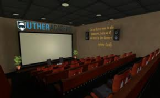
\includegraphics[]{UA}
    \caption{U.A. - aulă virtuală}
    \label{fig:imag4}
\end{figure}
    
\par Modul de prezentare generala nu diferă foarte mult de Secon Life. Studenții participa online la cursuri în clase virtuale. Procesul de învățare este supravegheat de instructori.

\section{iSocial}

\par iSocial este un mediu de învățare 3D, dezvoltat pe baza toolkit-ului pentru crearea lumilor virtuale OpenWonderland, creat pentru predarea de competențe sociale tinerilor diagnosticați cu autism (ASD). În acest scop, iSocial facilitează intracțiunea socială și oferă suport pentru dezvoltarea de competențe sociale într-un mediu sigur și complet controlat.
\par Localizarea geografica poate restricționa accesul la tratamentele și exercițiile necesare recuperării sociale a tinerilor afectați de ASD. iSocial este una dintre soluțiile rezolvării pozitive a acestei probleme.

\begin{figure}[h]
    \centering
    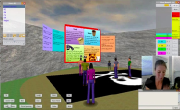
\includegraphics[]{IS}
    \caption{iSocial - panou informativ }
    \label{fig:imag5}
\end{figure}

\section{Tehnici/Tehnologii folosite}

\par Second Life (SL) este cea mai cunoscută și populară implementare a unei lumi virtuale. Deși nu este dezvoltată strict ca aplicație destinată instruirii in medii 3D, o parte însemnată a activităților desfașurate în Second Life sunt activități educcative.
\par Un studiul tehnologiilor folosite pentru dezvoltarea mediului Second Life este suficient pentru  identifica majoritatea bibliotecilor software foilosibile pentru dezvoltarea sub Linux a unei aplicații similare. S-a alcătuit o listă a tehnologiilor folosite pentru dezvoltarea SL.\ref{tab:SL_tech}
\begin{table}
      \begin{center}
            \begin{tabular}{|l|l|l|}
                \hline 
                \cline{2-3}
                $Denumire $ & $Bibliotecă/Ubuntu$ & $Utilizare$  \\ 
        	\hline
                $OpenGL$  	&  libGLU.so     	&  API pentru grfica 2D și 3D  \\
                $Zlib$   	&  libz.so     		&  Comprimare date  \\
                
                $OpenSSL$   &  libssl.so    	&  Protocoale de comunicare în rețea SSL și TLS  \\
                $OGG$   	&  libogg.so      	&  Format media audio-video  \\
                $PNG$   	&  libpng12.so      &  Imagini PNG  \\
                $GLib$   	&  libdbus-glib-1.so     &  Sistem de transmitere a mesajelor între procese  \\
                $GTK$   	&  libgtk2.0-dev 	&  GIMP toolkit  \\
                $OpenAL$   	&  libopenal-dev;libalut-dev	&  OpenAL - Biblitecă pt. redarea sunetului (audio) \\
                $Vorbis$   	&  libvorbis-dev 	&  Codec audio-video (API) \\
                $APACHE$   	&  libapr1-dev  	&  Apache portabele runtime  \\
                $JPEG$   	&  libopenjpeg.so;libjpeg.so &  Codec JPEG  \\
                $SDL$   	&  libsdl1.2-dev	&  Media Layer - faciliteaza accesul la periferice  \\
                $Boost$   	&  libboost-dev     &  Alternativa pentru C++ STL (+ comunicare în rețea) \\
                $JsonCpp$  	&  libjsoncpp-dev 	&  Interpretarea fișierelor Json (c++)  \\
            \hline
	    \end{tabular}
        \end{center}
    \caption{Tehnologii utilizabile petru dezvoltarea de medii 3D sub Linux}
    \label{tab:SL_tech}
\end{table}

\par Pentru dezvoltarea aplicației client SL se folosesc următoarele tehnologii: OpenGL pentru redarea graficii 3D, GTK pentru interfețele grafice, Boost și APACHE pentru schimbul de date în rețea între aplicația client și serverul lumii virtuale, Formatul de date JSON pentru structurarea datelor interschimbate în rețea între aplicația client și server, OpenAL pentru redarea sunetului și OGG/Vorbis ca și format/codec media și PNG/JPEG pentru redarea stocarea imaginilor. Codul sursă pentru serverul SL nu este open source.

\par O parte dintre aceste tehnologii sunt folosite pentru realizarea mediului de învățare 3D descris în această lucrare.
